\chapter{L'énergie dans la vie de tous les jours}\label{ch:g5:everyday-energy}

Un jouet mécanique file sur le plancher, ralentit et s'arrête ---
jusqu'à ce que tu le remontes. Une lampe de poche faiblit à mesure
que ses \omterm{def:g3:first-electric-circuit:battery}{piles} se fatiguent. Toi-même, tu n'en peux plus avant midi.
Tout ce qui bouge, brille, sonne ou réchauffe semble dépenser quelque
chose. La physique a un nom pour ce quelque chose, et c'est peut-être
le mot le plus important de tout ce livre~: l'\omterm{def:g5:everyday-energy:energy}{énergie}.

\section{Le quelque chose qui fait avancer les choses}

\begin{definition}[Énergie]\label{def:g5:everyday-energy:energy}
L'\emph{énergie}\index{énergie} est ce qu'il faut pour que les choses
se produisent~: mettre des objets en mouvement, les soulever, les
éclairer, les réchauffer, les faire sonner. Rien ne roule, ne brille
ni ne pousse sans qu'on y dépense de l'énergie --- et celui qui
dépense doit d'abord avoir de l'énergie à dépenser.
\end{definition}

\begin{definition}[Réservoirs d'énergie]\label{def:g5:everyday-energy:store}
Un \emph{réservoir d'énergie}\index{réservoir d'énergie} est tout ce
qui contient de l'\omterm{def:g5:everyday-energy:energy}{énergie} prête à servir. Les grands réservoirs de
tous les jours~: la \emph{nourriture} (le carburant de ton corps),
les \emph{combustibles} comme le bois et l'essence, les
\emph{\omterm{def:g3:first-electric-circuit:battery}{piles}} chargées, un \emph{ressort} remonté, l'eau retenue
\emph{en hauteur} derrière un barrage --- et le \emph{Soleil}
brûlant, qui déverse de l'\omterm{def:g5:everyday-energy:energy}{énergie} sur tout, toute la journée, et
gratuitement.
\end{definition}

\begin{example}[Trouve le réservoir]\label{ex:g5:everyday-energy:spot}
Derrière chaque chose qui avance, il y a un réservoir. La souris
mécanique qui file~: son ressort remonté. La lampe de poche~: ses
\omterm{def:g3:first-electric-circuit:battery}{piles}. La voiture~: le carburant de son réservoir. Toi~: ton
petit-déjeuner. Le voilier~: l'\omterm{def:g2:air-around-us:air}{air} en mouvement du \omterm{def:g2:air-around-us:wind}{vent}. Quand le
réservoir se vide --- ressort détendu, \omterm{def:g3:first-electric-circuit:battery}{piles} à plat, réservoir sec,
midi qui approche --- tout s'arrête.
\end{example}

\begin{remark}[Pas de nourriture, pas de marche]\label{rem:g5:everyday-energy:nofree}
Pendant des siècles, des inventeurs ont couru après des machines qui
tourneraient éternellement sans rien --- des roues qui se font
tourner elles-mêmes, des horloges qu'on ne remonte jamais. Toutes,
sans exception, ont échoué. Cet échec est l'une des leçons les plus
profondes de la physique~: l'\omterm{def:g5:everyday-energy:energy}{énergie} ne sort jamais du néant. Ce qui
marche est nourri --- trouve le réservoir, et tu comprends la
machine.
\end{remark}

\section{L'énergie change de forme}

\begin{example}[Les formes de l'énergie]\label{ex:g5:everyday-energy:forms}
L'\omterm{def:g5:everyday-energy:energy}{énergie} se montre sous différentes formes~: l'\omterm{def:g5:everyday-energy:energy}{énergie} de
\emph{mouvement} dans la balle qui roule et dans le \omterm{def:g2:air-around-us:wind}{vent} qui
souffle~; l'\omterm{def:g5:everyday-energy:energy}{énergie} \emph{lumineuse} qui \omterm{def:g1:floating-and-sinking:words}{coule} de la lampe et du
Soleil~; l'\omterm{def:g5:everyday-energy:energy}{énergie} \emph{thermique} dans tout ce qui est chaud~;
l'\omterm{def:g5:everyday-energy:energy}{énergie} \emph{électrique} qui voyage dans les fils~; l'\omterm{def:g5:everyday-energy:energy}{énergie}
\emph{en réserve} qui attend tranquillement dans la nourriture, les
combustibles, les ressorts et les objets soulevés. Un même quelque
chose, bien des formes.
\end{example}

\begin{proposition}[La chaîne d'énergie]\label{prop:g5:everyday-energy:chain}
Chaque fois qu'il se passe quelque chose, de l'\omterm{def:g5:everyday-energy:energy}{énergie} est puisée
dans un réservoir et transmise plus loin, en changeant le plus
souvent de forme en chemin. Elle n'est jamais créée à partir de
rien --- et jamais vraiment détruite non plus~: ce qu'une machine
«~consomme~» n'a été que transmis, et finit le plus souvent, tôt ou
tard, en douce chaleur répandue dans les environs.
\end{proposition}

\begin{method}[Lire une chaîne d'énergie]\label{met:g5:everyday-energy:read}
Pour comprendre n'importe quel appareil, suis sa chaîne~:
\begin{enumerate}
  \item trouver le \emph{réservoir} d'où vient l'\omterm{def:g5:everyday-energy:energy}{énergie}~;
  \item trouver le \emph{convertisseur} --- la pièce où l'\omterm{def:g5:everyday-energy:energy}{énergie}
        change de forme~;
  \item nommer les formes qui sortent --- la forme utile, et la
        chaleur qui fuit à côté.
\end{enumerate}
La lampe de poche, ainsi suivie~: \omterm{def:g3:first-electric-circuit:battery}{pile} (réservoir) $\to$ lampe
(convertisseur) $\to$ \omterm{def:g1:light-and-shadows:source}{lumière} (utile) $+$ un peu de chaleur (la
fuite --- touche la lampe).
\end{method}

\begin{omfigure}
\begin{tikzpicture}[scale=0.85]
  \node[draw, thick, omDef, font=\small, minimum width=2.5cm,
    minimum height=0.9cm] (a) at (1.4,0) {pile~: réservoir};
  \node[draw, thick, omMeth, font=\small, minimum width=2.5cm,
    minimum height=0.9cm] (b) at (5.4,0) {lampe~: convertisseur};
  \node[draw, thick, omThm, font=\small, minimum width=2.2cm,
    minimum height=0.9cm] (c) at (9.4,0.7) {lumière~: utile};
  \node[draw, thick, omExo, font=\small, minimum width=2.2cm,
    minimum height=0.9cm] (d) at (9.4,-0.7) {chaleur~: fuite};
  \draw[-Stealth, very thick] (a) -- (b);
  \draw[-Stealth, very thick] (b) -- (c);
  \draw[-Stealth, very thick] (b) -- (d);
\end{tikzpicture}

{\small La chaîne d'\omterm{def:g5:everyday-energy:energy}{énergie} de la lampe de poche~: l'\omterm{def:g5:everyday-energy:energy}{énergie} en
réserve devient de la \omterm{def:g1:light-and-shadows:source}{lumière} --- et un peu de chaleur s'échappe
toujours à côté.}
\end{omfigure}

\begin{example}[Des chaînes partout]\label{ex:g5:everyday-energy:chains}
Ton trajet du matin, suivi pas à pas~: le petit-déjeuner (réservoir)
$\to$ tes muscles (convertisseur) $\to$ mouvement du vélo $+$ chaleur
(tu la sens --- tu es tout rouge). Le parc éolien~: \omterm{def:g2:air-around-us:air}{air} en mouvement
$\to$ pales qui tournent $\to$ \omterm{def:g5:everyday-energy:energy}{énergie} électrique dans les fils $\to$
\omterm{def:g1:light-and-shadows:source}{lumière} dans ta lampe ce soir. Le barrage~: eau en hauteur $\to$ eau
qui tombe et fait tourner les turbines $\to$ \omterm{def:g5:everyday-energy:energy}{énergie} électrique. Les
longues chaînes ne sont que des courtes mises bout à bout~: forme
après forme après forme.
\end{example}

\begin{omfigure}
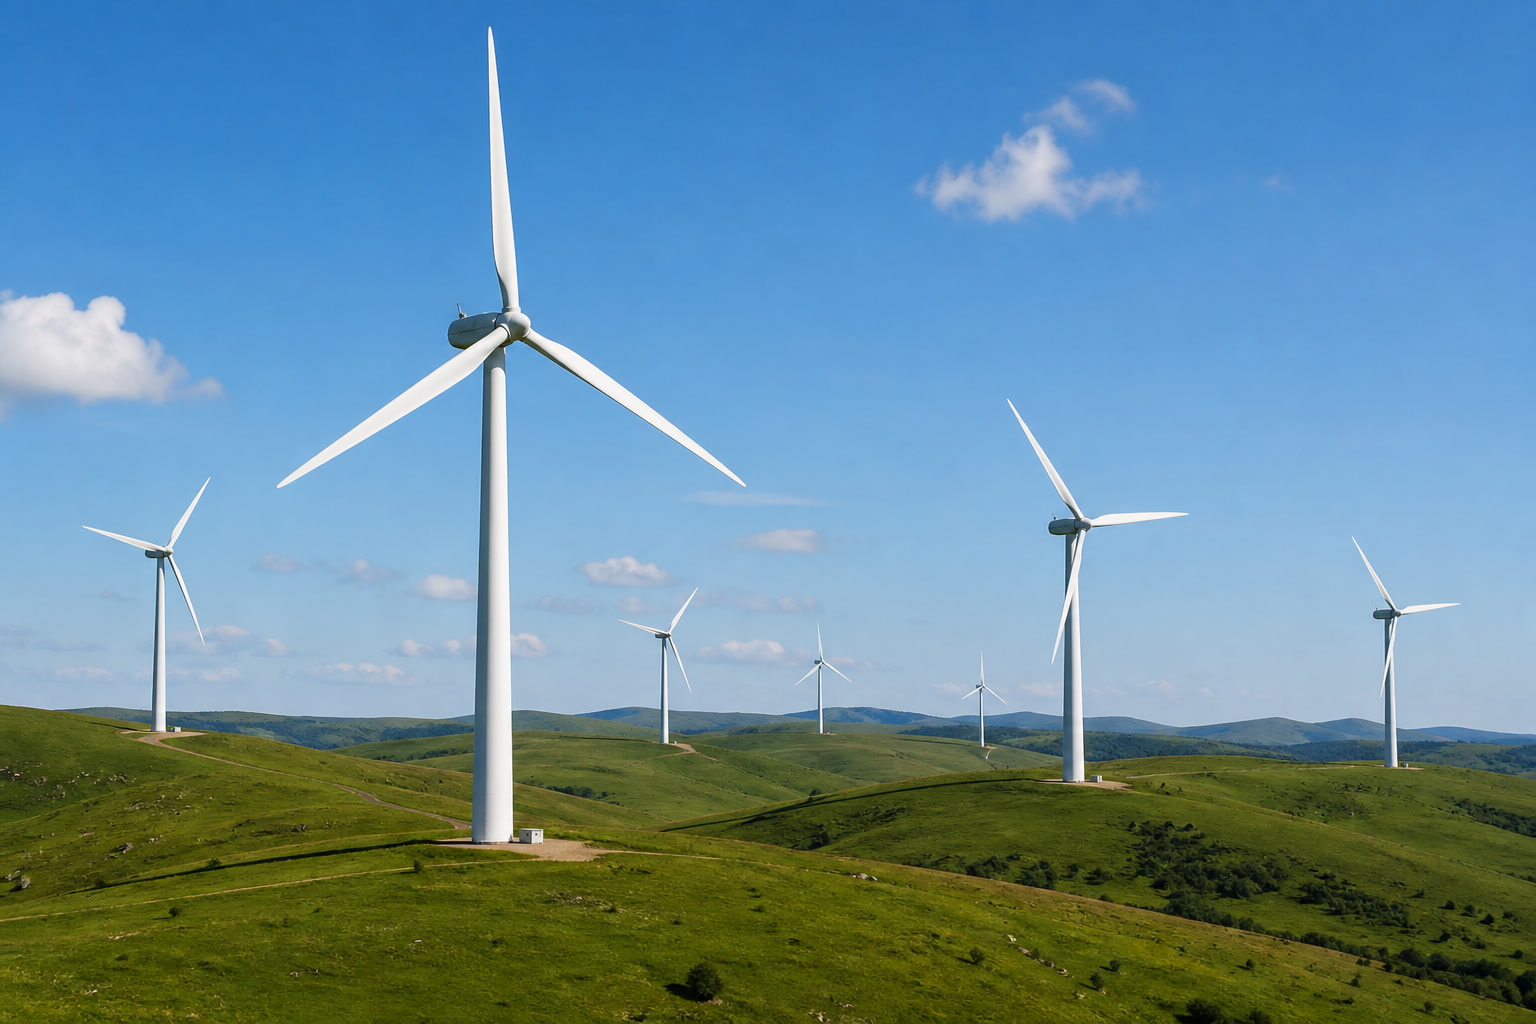
\includegraphics[width=0.58\linewidth]{images/book1/ai/g5-energy-windfarm.jpg}

{\small Une chaîne d'\omterm{def:g5:everyday-energy:energy}{énergie} que l'on voit depuis la route~: l'\omterm{def:g2:air-around-us:air}{air} en mouvement fait tourner les pales, et les turbines envoient de l'\omterm{def:g5:everyday-energy:energy}{énergie} électrique dans les fils.}
\end{omfigure}

\section{Le Soleil en bout de table}

\begin{example}[Presque toutes les chaînes partent du
Soleil]\label{ex:g5:everyday-energy:sun}
Remonte la plupart des chaînes et tu arrives au Soleil. Le
petit-déjeuner~? Des plantes l'ont fait pousser en captant la \omterm{def:g1:light-and-shadows:source}{lumière}
du Soleil~; tes céréales sont du soleil en boîte. Le \omterm{def:g2:air-around-us:wind}{vent}~? Le Soleil
réchauffe les terres inégalement, et l'\omterm{def:g2:air-around-us:air}{air} ainsi remué est le \omterm{def:g2:air-around-us:wind}{vent}
--- même les voiliers marchent donc à la \omterm{def:g1:light-and-shadows:source}{lumière} du Soleil. Le bois~?
De la \omterm{def:g1:light-and-shadows:source}{lumière} du Soleil mise en réserve par les arbres. L'eau haute
du barrage~? C'est le Soleil qui l'a soulevée~: il a fait s'\omterm{def:g2:ice-water-steam:evapcond}{évaporer}
la mer, et la vapeur est retombée en pluie sur les montagnes. Les
panneaux solaires, eux, se contentent de sauter les intermédiaires.
\end{example}

\begin{omfigure}
\begin{tikzpicture}[scale=0.85]
  \fill[omThm] (0.9,3.2) circle (0.45);
  \foreach \a in {0,30,...,330} {
    \draw[omThm] (0.9,3.2) ++(\a:0.62) -- ++(\a:0.26);
  }
  \node[below, font=\small] at (0.9,2.5) {le Soleil};
  \node[draw, thick, omMeth, font=\small] (p) at (4.3,3.2) {plantes};
  \node[draw, thick, omDef, font=\small] (f) at (7.2,3.2) {nourriture};
  \node[draw, thick, omMeth, font=\small] (m) at (9.9,3.2) {muscles};
  \node[draw, thick, omMeth, font=\small] (w) at (4.3,1.4)
    {air réchauffé et remué};
  \node[draw, thick, omDef, font=\small] (v) at (8.3,1.4)
    {vent et voiles};
  \draw[-Stealth, very thick] (1.6,3.2) -- (p);
  \draw[-Stealth, very thick] (p) -- (f);
  \draw[-Stealth, very thick] (f) -- (m);
  \draw[-Stealth, very thick] (1.35,2.75) -- (w);
  \draw[-Stealth, very thick] (w) -- (v);
\end{tikzpicture}

{\small Deux chaînes remontées jusqu'à leur source~: le
petit-déjeuner et le \omterm{def:g2:air-around-us:wind}{vent} commencent tous deux au Soleil.}
\end{omfigure}

\begin{remark}[Un mot que nous aiguiserons]\label{rem:g5:everyday-energy:promise}
Pour l'instant, l'\omterm{def:g5:everyday-energy:energy}{énergie} est une histoire bien racontée~: des
réservoirs, des formes, des chaînes. Peut-elle être \emph{mesurée},
comme la longueur en \omterm{def:g2:measuring-length:units}{mètres} et la \omterm{def:g3:measuring-mass:mass}{masse} en \omterm{def:g3:measuring-mass:units}{grammes}~? Oui ---
l'\omterm{def:g5:everyday-energy:energy}{énergie} a son \omterm{def:g2:measuring-length:measure}{unité} propre et sa comptabilité exacte, et elles
arrivent plus loin dans ce livre, une fois que tu auras rencontré
comme il faut la vitesse et la \omterm{def:g2:pushes-and-pulls:force}{force}. Les chaînes que tu suis cette
année sont la carte~; les nombres viendront l'habiter.
\end{remark}

\section{Exercices}

\begin{exercise}[$\star$]\label{exo:g5:everyday-energy:1}
Qu'est-ce que l'\omterm{def:g5:everyday-energy:energy}{énergie}, selon les mots de ce chapitre~? Cite quatre
choses qui ne peuvent pas se produire sans elle.
\end{exercise}

\begin{exercise}[$\star$]\label{exo:g5:everyday-energy:2}
Trouve le réservoir~: une souris mécanique qui file~; \ un
cycliste~; \ un feu de camp~; \ un voilier~; \ une lampe de poche.
\end{exercise}

\begin{exercise}[$\star$]\label{exo:g5:everyday-energy:3}
Cite cinq formes d'\omterm{def:g5:everyday-energy:energy}{énergie}, avec un exemple de chacune tiré de ta
propre journée.
\end{exercise}

\begin{exercise}[$\star$]\label{exo:g5:everyday-energy:4}
Suis la chaîne d'\omterm{def:g5:everyday-energy:energy}{énergie} d'un grille-pain, comme dans
\cref{met:g5:everyday-energy:read}~: réservoir, convertisseur, formes
qui sortent.
\end{exercise}

\begin{exercise}[$\star$]\label{exo:g5:everyday-energy:5}
Suis la chaîne qui va du lac d'un barrage à ta lampe de lecture, ce
soir.
\end{exercise}

\begin{exercise}[$\star$]\label{exo:g5:everyday-energy:6}
Un téléphone «~meurt~». Qu'est-ce qui s'est réellement épuisé~? Où
est passée cette \omterm{def:g5:everyday-energy:energy}{énergie}, d'après la proposition de la chaîne~?
\end{exercise}

\begin{exercise}[$\star$]\label{exo:g5:everyday-energy:7}
Pourquoi un ordinateur portable devient-il chaud par-dessous pendant
que tu t'en sers~? Quel maillon de la chaîne se manifeste~?
\end{exercise}

\begin{exercise}[$\star$]\label{exo:g5:everyday-energy:8}
Montre qu'un voilier marche à la \omterm{def:g1:light-and-shadows:source}{lumière} du Soleil, en remontant sa
chaîne étape par étape.
\end{exercise}

\begin{exercise}[$\star\star$]\label{exo:g5:everyday-energy:9}
Un inventeur annonce une lampe qui «~n'a besoin ni de \omterm{def:g3:first-electric-circuit:battery}{pile}, ni de
prise, ni de combustible --- elle brille tout simplement pour
toujours~». Quelle leçon de \cref{rem:g5:everyday-energy:nofree} son
annonce défie-t-elle~? Quelle question faut-il poser en premier à
l'inventeur~?
\end{exercise}

\begin{exercise}[$\star\star$]\label{exo:g5:everyday-energy:10}
Une balle en caoutchouc lâchée à hauteur d'épaule rebondit de moins
en moins haut et finit par rester immobile. «~Son \omterm{def:g5:everyday-energy:energy}{énergie} est
détruite~», dit Léo. Sers-toi de \cref{prop:g5:everyday-energy:chain}
pour défendre une meilleure fin de l'histoire --- sous quelle forme
finale l'\omterm{def:g5:everyday-energy:energy}{énergie} des rebonds s'est-elle glissée~?
\end{exercise}

\begin{exercise}[$\star\star$]\label{exo:g5:everyday-energy:11}
Certaines maisons chauffent leur eau dans des panneaux noirs posés
sur le toit~; certaines cuisinent avec la \omterm{def:g1:light-and-shadows:source}{lumière} du Soleil et des
miroirs courbes~; les cellules solaires fabriquent de l'électricité à
partir de la \omterm{def:g1:light-and-shadows:source}{lumière} du jour. Explique la phrase «~les panneaux
solaires se contentent de sauter les intermédiaires~» de
\cref{ex:g5:everyday-energy:sun}~: quels intermédiaires se tiennent
entre le Soleil et la chaleur d'un feu de bois~?
\end{exercise}
